\documentclass[11pt]{article}

\usepackage[a4paper,margin=24mm]{geometry}
\usepackage[T1]{fontenc}
\usepackage[utf8]{inputenc}
\usepackage{lmodern}
\usepackage{microtype}
\usepackage{amsmath,amssymb}
\usepackage{booktabs}
\usepackage{graphicx}
\usepackage{array}
\usepackage{enumitem}
\usepackage{xcolor}
\usepackage[hidelinks]{hyperref}

\definecolor{forest}{HTML}{31572C}
\definecolor{orange}{HTML}{C44900}
\setlength{\parindent}{0pt}
\setlength{\parskip}{0.55em}
\setlist{nosep,leftmargin=*}
\renewcommand{\arraystretch}{1.13}

\title{\textbf{Five-Seed Evaluation of Rule-Based DAgger\\on Generated CartPole Demonstrations}}
\author{Experimental supplement to \emph{Experimental Analysis of DAgger}\\
Nowshin Tabassum, Intesur Ahmed, and Md. Rakibul Hassan}
\date{21 August 2026}

\begin{document}
\maketitle

\begin{abstract}
This report evaluates DAgger using the generated CartPole CSV and the rule-based expert specified in the project plan. Five independent learners (training seeds 0--4) were initialized from the same 1,500 rule-expert transitions and then trained through five online mixed-policy DAgger rounds. The rule expert labeled every state visited online. Checkpoints were evaluated without expert assistance on the same 20 episodes used by the separate PPO-expert baseline. Round-0 return was $175.89\pm47.78$ across seeds (mean $\pm$ sample standard deviation; 95\% Student-$t$ interval [116.57, 235.21]). Round 1 improved to $489.11\pm7.21$ (95\% interval [480.16, 498.06]), but no seed was yet exactly at the 500-step ceiling. From round 2 through round 5, all five learners scored 500 on every checkpoint evaluation, and all repeated 500 on a separate final test. Under the matched protocol, the PPO-expert baseline reached the ceiling at round 1, one round earlier, while both expert pipelines had identical final return. The comparison is descriptive because the initial state distributions and expert-generation processes differ.
\end{abstract}

\section{Purpose and scope}

The previous report measured a library DAgger baseline in which a new proximal policy optimization (PPO) expert was trained for every seed. The present experiment answers a separate question: \emph{What happens when DAgger starts from the project's generated CSV and queries the PDF's analytic rule during online collection?}

This is the primary rule-expert CartPole path. It does not train a PPO expert and it does not import the PPO policy. The PPO results are read only after both experiments finish, for plotting and descriptive comparison. This report still does not cover Stanford OCR, label-budgeted querying, data-retention ablations, or partial observability.

\section{Data provenance and expert}

The initial file is \texttt{cartpole\_expert\_demonstrations.csv}. It contains 50,000 transitions from 100 CartPole-v1 episodes generated with seeds 0--99. Every source episode reached the 500-step horizon. The dataset SHA-256 is
\begin{center}
\small\texttt{d2fb810a58850fe5af3983bccd39e6bb55fb1e591a013b6b7505947d3bd838a7}.
\end{center}

The expert is the formula stated in the project PDF:
\[
\pi^*(x,\dot{x},\theta,\dot{\theta})
=\mathbb{1}\!\left[\theta+0.6\dot{\theta}+0.02\dot{x}>0\right].
\]
The implementation recomputed this formula for every selected CSV row and stopped if a stored action disagreed. All 1,500 selected actions passed this check. The subset contained exactly 750 left and 750 right actions.

The fixed CSV is used only for initialization. DAgger cannot be performed solely by repeatedly training on that file: later rounds must run the current learner, visit learner-influenced states, query the rule on those states, and append the new labels.

\section{Methodology}

\subsection{Why 1,500 of the 50,000 CSV rows were selected}

Round 0 uses complete CSV episodes 0, 1, and 2, totaling $3\times500=1{,}500$ transitions. This matches the PPO-library baseline's first-round label count. Training on all 50,000 rows would give the rule learner over 33 times more initial labels and would make the curves unsuitable for a label-matched comparison. The remaining CSV rows are preserved and can later be studied as an initial-dataset-size ablation.

All five learner seeds use the same 1,500-row initial subset. Therefore, round-0 variation in this experiment comes from learner initialization and optimization, not from changing the fixed offline dataset.

\subsection{Learner and update}

The learner uses \texttt{imitation.algorithms.bc.BC} and its default \texttt{FeedForward32Policy}: two shared 32-unit tanh hidden layers and a two-action output. Optimization uses Adam, learning rate $10^{-3}$, batch size 32, and four behavior-cloning epochs after every round. All prior labeled states are retained. These settings match the learner architecture, optimizer, batch size, update epochs, and retention rule in the PPO-library experiment.

For behavior cloning, each training item is $(s,\pi^*(s))$. The package's data loader also requires shape-compatible \texttt{next\_obs} and \texttt{done} fields, although they do not enter the BC objective. The recorded scientific inputs remain the observation and rule-expert action.

\subsection{Online DAgger collection}

At online round $i\in\{1,2,3,4,5\}$, the collection policy is
\[
\pi_i=\beta_i\pi^*+(1-\beta_i)\hat\pi_i,
\qquad \beta_i=0.5^i.
\]
At every visited state, the system records the observation, expert label, learner action, physically executed action, expert-control coin, reward, termination flag, truncation flag, episode ID, and timestep. The expert label is retained regardless of which policy controls the environment. This is standard dense-label DAgger.

Collection continues until both conditions are satisfied: at least three \emph{complete} episodes and at least 500 transitions. Early learner-influenced episodes can fail before 500 steps. Consequently, a round does not always contain 1,500 transitions. This stopping rule is the same logical rule used by the library baseline; 1,500 occurs when all three episodes reach the horizon.

After collection, the new rule labels are appended to all earlier labels, the learner is trained for four epochs on the aggregate, and the new checkpoint is evaluated. Round 0 denotes the checkpoint after training on the three CSV episodes. Round 1 denotes the checkpoint after the first online collection with $\beta_1=0.5$.

\subsection{Independent seeds and fixed evaluation}

The full learner and online-collection procedure was repeated with training seeds 0--4. A training seed changes neural initialization, behavior-cloning minibatches, CartPole collection states, and expert/learner mixing coins. The rule expert remains deterministic and is not retrained.

After every checkpoint, the learner acts alone and deterministically for 20 episodes. No expert actions are permitted during evaluation. A fresh environment is reconstructed with common seed 40,000 at every round for all five learners. A separate final test uses common seed 30,000. The rule expert is evaluated with seed 10,000. The reset sequence was matched to the PPO-library evaluator, and the episode rewards were saved individually.

\begin{table}[ht]
\centering
\caption{Matched experimental configuration.}
\small
\begin{tabular}{@{}p{0.39\linewidth}p{0.52\linewidth}@{}}
\toprule
Item & Rule-expert setting \\
\midrule
Environment & Gymnasium CartPole-v1; ceiling 500 \\
Training seeds & 0, 1, 2, 3, 4 \\
Initial data & CSV episodes 0--2; 1,500 labels \\
Expert & Deterministic PDF formula \\
Learner & FeedForward32Policy, hidden layers [32,32] \\
Update & Adam, LR $10^{-3}$, batch 32, 4 epochs/round \\
Retention & Complete aggregate of all past labels \\
Mixing & $\beta_i=0.5^i$ \\
Online stopping rule & At least 3 complete episodes and 500 steps \\
Round evaluation & 20 episodes, common seed 40,000 \\
Final evaluation & 20 episodes, common seed 30,000 \\
\bottomrule
\end{tabular}
\end{table}

\subsection{Uncertainty calculation}

For each checkpoint, one value per training seed is first computed by averaging its 20 episode returns. Across-seed uncertainty is then
\[
\bar R_i\ \pm\ t_{0.975,4}\frac{s_i}{\sqrt{5}},
\qquad t_{0.975,4}=2.7764,
\]
where $s_i$ is the sample standard deviation of the five training-seed means. This 95\% Student-$t$ interval describes variation from rerunning learner training. It is different from the standard deviation among evaluation episodes for one saved learner.

\section{Rule-expert results}

\subsection{Raw checkpoint returns}

\begin{table}[ht]
\centering
\caption{Measured mean return over the 20 fixed round-evaluation episodes.}
\small
\begin{tabular}{@{}crrrrrr@{}}
\toprule
Seed & R0 & R1 & R2 & R3 & R4 & R5 \\
\midrule
0 & 225.05 & 484.75 & 500.00 & 500.00 & 500.00 & 500.00 \\
1 & 184.70 & 478.45 & 500.00 & 500.00 & 500.00 & 500.00 \\
2 & 125.30 & 494.35 & 500.00 & 500.00 & 500.00 & 500.00 \\
3 & 127.20 & 493.75 & 500.00 & 500.00 & 500.00 & 500.00 \\
4 & 217.20 & 494.25 & 500.00 & 500.00 & 500.00 & 500.00 \\
\bottomrule
\end{tabular}
\end{table}

Round 0 varies from 125.30 to 225.05. Round 1 is much stronger, but every seed remains below 500. Round 2 is the first checkpoint where all five seeds obtain exactly 500, and that ceiling remains through round 5.

\subsection{Aggregate learning curve}

\begin{table}[ht]
\centering
\caption{Across-seed return and data-collection summary. Labels and disagreement are means across the five runs.}
\small
\begin{tabular}{@{}crrrrrr@{}}
\toprule
R & $\beta$ & Cum. labels & Return & Seed SD & 95\% CI & Disagree \\
\midrule
0 & 1.0000 & 1,500.0 & 175.89 & 47.78 & [116.57,235.21] & -- \\
1 & 0.5000 & 2,642.8 & 489.11 & 7.21 & [480.16,498.06] & 19.67\% \\
2 & 0.2500 & 4,093.2 & 500.00 & 0.00 & [500.00,500.00] & 11.74\% \\
3 & 0.1250 & 5,593.2 & 500.00 & 0.00 & [500.00,500.00] & 10.76\% \\
4 & 0.0625 & 7,093.2 & 500.00 & 0.00 & [500.00,500.00] & 4.19\% \\
5 & 0.0313 & 8,593.2 & 500.00 & 0.00 & [500.00,500.00] & 2.35\% \\
\bottomrule
\end{tabular}
\end{table}

The paired round-0-to-round-1 improvement is 313.22 return points on average, with sample standard deviation 51.27 and 95\% interval [249.56, 376.88]. This supports a large, consistent improvement after the first online DAgger collection. Round 1 averaged 1,142.8 new labels because several mixed-policy episodes ended early; round 2 averaged 1,450.4. Rounds 3--5 added exactly 1,500 labels because all three collection episodes reached the horizon in every run.

The realized expert-control fractions were 0.490, 0.261, 0.136, 0.0628, and 0.0331 for rounds 1--5, close to the intended probabilities 0.5, 0.25, 0.125, 0.0625, and 0.03125. The differences are normal finite-sample coin variation. The mean pre-update learner/expert action disagreement declined from 19.67\% in round 1 to 2.35\% in round 5, although it was not strictly monotonic at every intermediate seed and round.

\begin{figure}[ht]
\centering
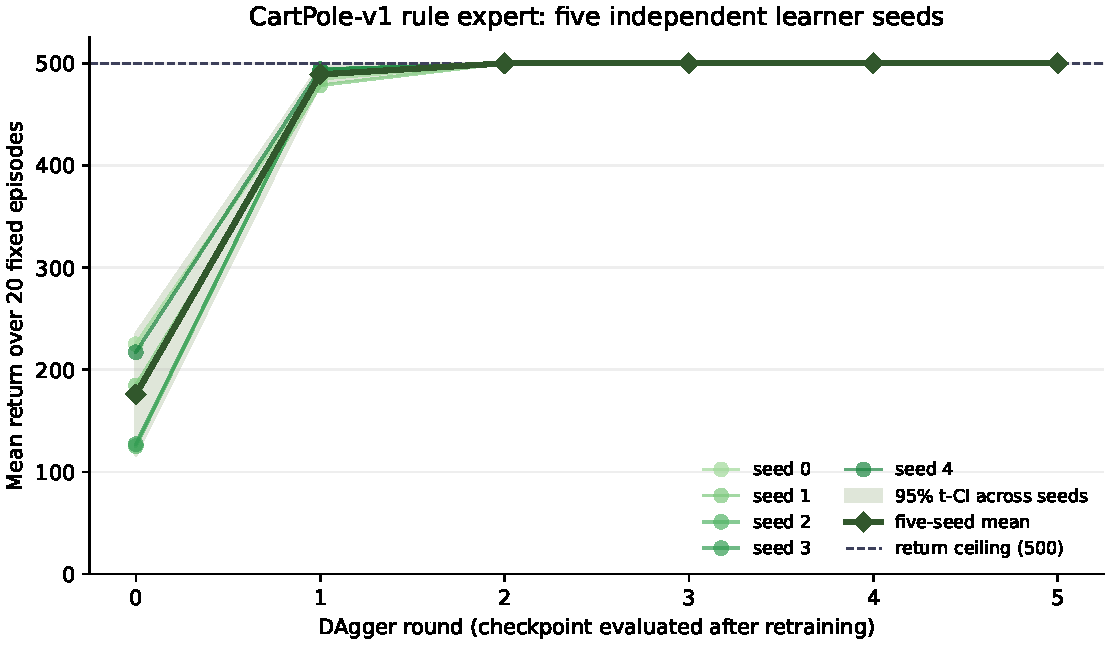
\includegraphics[width=\linewidth]{../analysis/rule_dagger_learning_curve.pdf}
\caption{Rule-expert DAgger learning curves for five independently trained learners. The shaded band is the two-sided 95\% Student-$t$ interval over training-seed means.}
\label{fig:rulecurve}
\end{figure}

\subsection{Expert and final checks}

The deterministic rule expert scored $500.00\pm0.00$ across its 20 evaluation episodes. Each final rule-DAgger learner scored $500.00\pm0.00$ on the separate 20-episode final evaluation. Therefore, the final across-seed mean is 500, its observed seed standard deviation is 0, and all 100 final learner episode evaluations reached the horizon.

Actual total labels differed because the stopping rule retains complete episodes: 8,326, 8,752, 8,660, 8,609, and 8,619 labels for seeds 0--4. The mean was 8,593.2, sample standard deviation 159.68, and 95\% interval [8,394.93, 8,791.47]. This variation is expected and is reported rather than silently treating the intended budget as the realized count.

\section{Comparison with the PPO-expert baseline}

Both studies use training seeds 0--4, a [32,32] learner, four BC epochs per round, full aggregation, the same $\beta$ schedule, learner-only deterministic evaluation, and the same 20 evaluation episode sequences. These controls make the curves directly useful as pipeline-level comparisons.

\begin{table}[ht]
\centering
\caption{Descriptive five-seed mean-return comparison. Difference is rule minus PPO.}
\small
\begin{tabular}{@{}crrr@{}}
\toprule
Round & Rule expert & PPO expert & Difference \\
\midrule
0 & 175.89 & 191.29 & $-15.40$ \\
1 & 489.11 & 500.00 & $-10.89$ \\
2 & 500.00 & 500.00 & 0.00 \\
3 & 500.00 & 500.00 & 0.00 \\
4 & 500.00 & 500.00 & 0.00 \\
5 & 500.00 & 500.00 & 0.00 \\
\bottomrule
\end{tabular}
\end{table}

At round 0, the rule interval [116.57,235.21] and PPO interval [70.61,311.97] overlap widely, so the modest difference in means should not be interpreted as reliable superiority. At round 1, all PPO learners are already at 500, whereas rule learners average 489.11 and range from 478.45 to 494.35. At round 2, both pipelines have all five learners at the ceiling and remain indistinguishable by standard return thereafter.

\begin{figure}[ht]
\centering
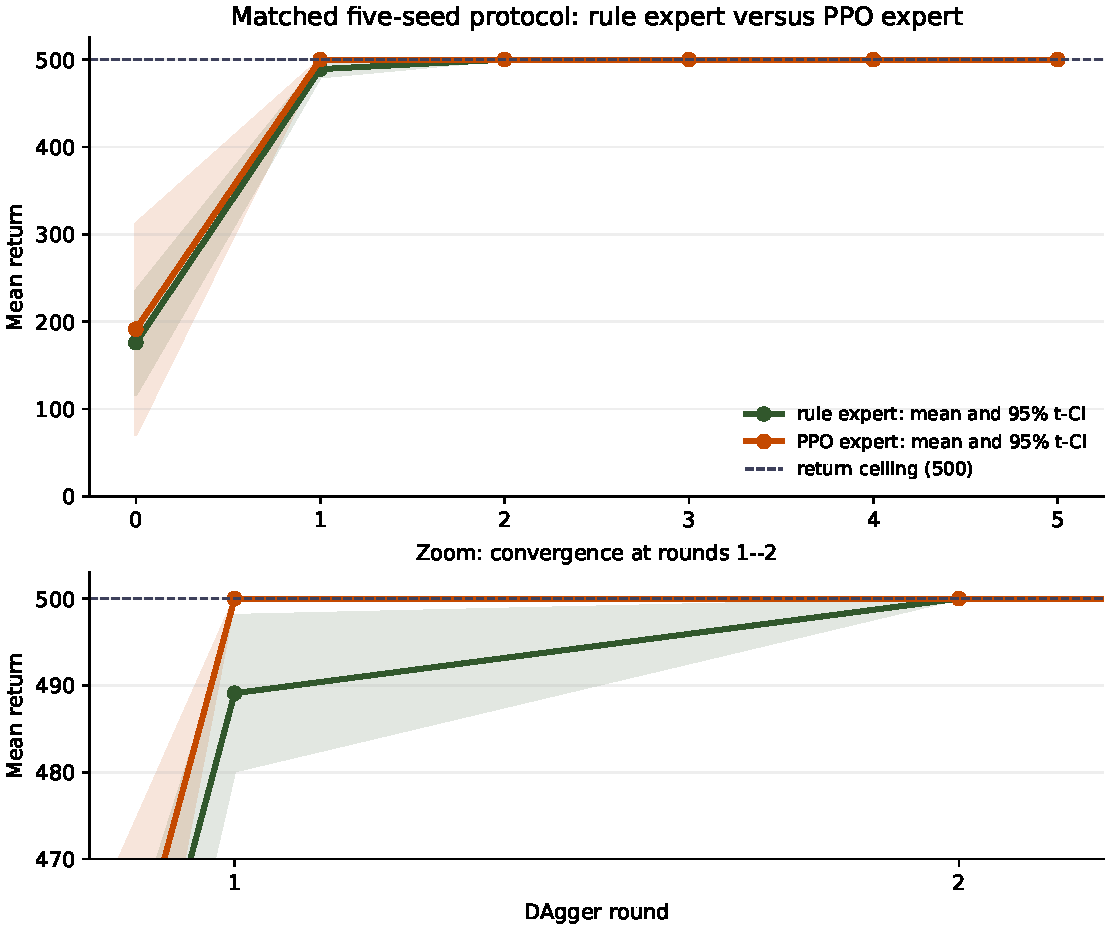
\includegraphics[width=\linewidth]{../analysis/rule_vs_ppo_comparison.pdf}
\caption{Rule-expert versus PPO-expert learning curves. The upper panel shows the full return range; the lower panel enlarges rounds 1--2 so the rule pipeline's one-round-later ceiling is visible. Bands are separate 95\% intervals across five training-seed means.}
\label{fig:comparison}
\end{figure}

The PPO pipeline reached the measured ceiling after 3,000 DAgger labels. The rule pipeline reached it after an average of 4,093.2 cumulative labels. However, this is not a complete cost comparison: every PPO run first trained an expert for 51,200 environment steps, while the analytic rule required no expert training. PPO used fewer learner labels in this experiment, whereas the rule expert was far cheaper to construct.

\subsection{Why this is not an isolated causal comparison of expert quality}

The pipelines differ in more than the formula. Rule round 0 uses the same fixed CSV episodes for every seed; PPO round 0 recollects states from a separately trained PPO expert and training environment for each seed. The PPO collector is library-managed, while the rule collector is an audited custom implementation that uses the same stopping logic and BC package. Consequently, Figure~\ref{fig:comparison} answers which complete pipeline reached the ceiling sooner under the matched settings. It does not prove that PPO labels are intrinsically better than rule labels.

An isolated expert-source ablation should collect one common state set, label every state with both experts, hold learner initialization and minibatch ordering fixed, and compare expert disagreement and downstream return. That is an appropriate next experiment if the report needs a causal expert-quality claim.

\section{Interpretation and limitations}

The rule-based expert successfully generates a usable initial dataset and supports online DAgger. Multiple learner seeds produce different early results, but aggregation steadily reduces both performance variation and action disagreement. Unlike the PPO baseline, the rule learner is not perfectly solved at round 1; nevertheless, every seed reaches the ceiling by round 2 and remains there.

Several limits constrain this conclusion:
\begin{enumerate}
  \item The five seeds and two fixed 20-episode sequences are evidence, not a universal guarantee over all seeds and initial states.
  \item Return 500 creates a ceiling effect. Later checkpoints may differ in robustness even when standard CartPole-v1 cannot distinguish them.
  \item Only 1,500 CSV rows were used for matched initialization. Training on all 50,000 rows should be reported as a separate dataset-size ablation, not mixed into this curve.
  \item This is dense-label DAgger. It queries the rule at every visited state and therefore does not test the project's label-budget novelty.
  \item The comparison includes different expert-generation and round-0 state-distribution processes; it is descriptive at the pipeline level.
  \item Neither result supplies evidence for OCR, retention strategies, uncertainty querying, or recurrent partial-observability experiments.
\end{enumerate}

\section{Reproducibility and artifacts}

From \texttt{Final Project/rule\_based\_cartpole}, run:
\begin{verbatim}
../imitation_library_cartpole/.venv/bin/python \
  run_five_seed_study.py
MPLCONFIGDIR=/tmp/matplotlib-rl-project \
  ../imitation_library_cartpole/.venv/bin/python \
  analyze_multiseed_study.py
\end{verbatim}

The output contains five raw JSON result files, 30 policy checkpoints plus final copies, 30 compressed round datasets, per-seed and aggregate CSV tables, both graphs in PDF/PNG formats, execution logs, and this LaTeX source/PDF. Software versions were NumPy 1.26.4, Gymnasium 0.29.1, PyTorch 2.2.2+cpu, Stable-Baselines3 2.2.1, and imitation 1.0.1.

\section{Conclusion}

DAgger was successfully run on the generated rule-based CartPole data. The correct measured statement is: \emph{across five independent learner seeds, rule-expert DAgger averaged 175.89 at round 0, 489.11 at round 1, and reached the return ceiling of 500 for every seed from round 2 onward}. The matched PPO pipeline reached the same ceiling one round earlier, but both produced final return 500. The rule result is especially valuable for the main project because its dataset and online labels follow the expert formula stated in the supplied PDF.

\begin{thebibliography}{9}
\bibitem{ross2011}
S. Ross, G. Gordon, and J. A. Bagnell,
``A Reduction of Imitation Learning and Structured Prediction to No-Regret Online Learning,''
\emph{Proceedings of AISTATS}, 2011.
\end{thebibliography}

\end{document}
